\documentclass[12pt, a4paper]{scrartcl}

% !TeX root = ../ITS_WiSe_202021_Hausarbeit_969272.tex
\usepackage{a4wide}

\usepackage[utf8]{inputenc}

%\usepackage[ngerman]{babel}
\usepackage[english]{babel}

\usepackage[T1]{fontenc}
\usepackage{palatino}

\usepackage{graphicx}
\usepackage{caption}
\usepackage{url}
\usepackage{tocloft}
\usepackage{acronym}

\usepackage{mathpazo}
\usepackage{amsmath}
\usepackage{amsfonts}
\usepackage{adjustbox}

%\usepackage{subcaption}

\usepackage{hhline}
\usepackage{amssymb}
\usepackage{floatflt}
\usepackage{setspace}
\usepackage{float}
\usepackage{color}
\usepackage{listings}
\usepackage{array}
\usepackage{scrhack}
\usepackage{xcolor}
\usepackage{wrapfig}
\usepackage{hyperref}
\usepackage{url}
\usepackage{lmodern}
\usepackage{multirow}
\usepackage{subcaption}
\usepackage{cleveref}
\usepackage{lipsum}


% !TeX root = ../ITS_WiSe_202021_Hausarbeit_969272.tex
%%%%%%%%%%%%%%%%%%%%%%%%%%%%%%%%%%%%%%%%%%%%%%%%%%%%%%%%%%%%%%%%%%%%%%%%
% Data about you and the Document%
%%%%%%%%%%%%%%%%%%%%%%%%%%%%%%%%%%%%%%%%%%%%%%%%%%%%%%%%%%%%%%%%%%%%%%%%

% % Main Title of Document:
\newcommand{\myMaintitle}{ITS - Klausurersatzleistung}

% % Sub Title of DocInput:
\newcommand{\mySubtitle}{Developing holistic software solutions through integration of existing individual solutions.}

% % Ihr Name:
\newcommand{\myName}{Henrik Gerdes}

% % Matrikelnummer:
\newcommand{\myMatrikel}{MatNr: 969272}

% % Ihr Geburtsort:
\newcommand{\brith}{Osnabrück}

% % Ihr Geburtsort:
\newcommand{\place}{Osnabrück}

% % Ihr Abgabedatum:
\newcommand{\submission}{\today}

% % Ihr Abgabedatum:
\newcommand{\mycourse}{IT - Sicherheit}

% % Name des Betreuers/Erstprüfenden:
\newcommand{\fistSupervisor}{Dennis Ziegenhagen}
\newcommand{\secSupervisor}{Prof.\ Elke Pulvermüller}

% % In welchem Semester befinden Sie sich?
\newcommand{\mySemester}{6. Semester}

\title{\myMaintitle}

\author{\myName}
% !TeX root = ../ITS_WiSe_202021_Hausarbeit_969272.tex
% % Zeilenabstand im Haupttext auf anderthalb-zeilig setzen
%\linespread{1.25}\selectfont

% Line spacing
%\onehalfspacing{}

%Pfad für Grafiken
\graphicspath{{fig/}}

%Styleregeln
\widowpenalty10000 % Vermeidet einzelne Zeilen eines Absatzes zu Beginn einer Seite
\clubpenalty10000 % Vermeidet einzelne Zeilen eines Absatzes am Ende einer Seite
\addtocontents{toc}{\protect\sloppy}
\setcounter{tocdepth}{3}


% % \sloppy bewirkt, dass Latex beim Blocksatz nicht über den rechten Rand hinausschreibt.
% % und dafür größere Lücken in einer Zeile in Kauf nimmt
\sloppy

% % Setzt Dokumenteigenschaften für PDFs, wenn das Paket 'hyperref' geladen wurde.
\hypersetup{pdftitle=\myMaintitle,pdfauthor=\myName,bookmarksopen=true}

%Source for picture captions
\newcommand{\source}[1]{\caption*{Source: {#1}} }

\newcommand{\code}[1]{\texttt{#1}}

\newcommand{\myparagraph}[1]{\paragraph{#1}\mbox{}\\}

\newcommand{\RM}[1]{\MakeUppercase{\romannumeral{} #1{}}}

\newcommand{\HRule}{\rule{\linewidth}{0.5mm}} % Defines a new command for horizontal


\definecolor{dkgreen}{rgb}{0,0.6,0}
\definecolor{gray}{rgb}{0.5,0.5,0.5}
\definecolor{mauve}{rgb}{0.58,0,0.82}

\lstset{ %
  language=Java,                  % the language of the code
  basicstyle=\footnotesize,       % the size of the fonts that are used for the code
  numbers=left,                   % where to put the line-numbers
  numberstyle=\tiny\color{gray},  % the style that is used for the line-numbers
  stepnumber=1,                   % the step between two line-numbers. If it's 1, each line
                                  % will be numbered
  numbersep=5pt,                  % how far the line-numbers are from the code
  backgroundcolor=\color{white},  % choose the background color. You must add \usepackage{color}
  showspaces=false,               % show spaces adding particular underscores
  showstringspaces=false,         % underline spaces within strings
  showtabs=false,                 % show tabs within strings adding particular underscores
  frame=single,                   % adds a frame around the code
  rulecolor=\color{black},        % if not set, the frame-color may be changed on line-breaks within not-black text (e.g. commens (green here))
  tabsize=4,                      % sets default tabsize to 2 spaces
  captionpos=b,                   % sets the caption-position to bottom
  breaklines=true,                % sets automatic line breaking
  breakatwhitespace=false,        % sets if automatic breaks should only happen at whitespace
  title=\lstname,                 % show the filename of files included with \lstinputlisting;
                                  % also try caption instead of title
  keywordstyle=\color{blue},          % keyword style
  commentstyle=\color{dkgreen},       % comment style
  stringstyle=\color{mauve}         % string literal style
}

%%%%%%%%%%%%%%%%%%%%%%%%%%%%%%%%%%%%%%%%%%%%%%%%%%%%%%%%%%%%%%%%%%%%%%%%%%%%%%%%%%%%%%%%%
%Examples
%%%%%%%%%%%%%%%%%%%%%%%%%%%%%%%%%%%%%%%%%%%%%%%%%%%%%%%%%%%%%%%%%%%%%%%%%%%%%%%%%%%%%%%%%
% \pdfmarkupcomment[markup=Squiggly,color=green]{with pdfcomment}{move to the front}.
% \pdfmarkupcomment[markup=StrikeOut,color=red]{stupid}{replace stupid with funny}
% \pdfmarkupcomment[markup=Highlight,color=yellow]{Of course, you can highlight complete sentences.}{Highlight}
% \pdfcomment[icon=Note,color=blue]{insert graphic!}

\begin{document}

\pagenumbering{gobble}
% !TeX root = ../ITS_WiSe_202021_Hausarbeit_969272.tex
%%%%%%%%%%%%%%%%%%%%%%%%%%%%%%%%%%%%%%%%%
% Academic Title Page
% LaTeX Template
% Version 2.0 (17/7/17)
%
% This template was downloaded from:
% http://www.LaTeXTemplates.com
%
% Original author:
% WikiBooks (LaTeX - Title Creation) with modifications by:
% Vel (vel@latextemplates.com)
%
% License:
% CC BY-NC-SA 3.0 (http://creativecommons.org/licenses/by-nc-sa/3.0/)
%
% Instructions for using this template:
% This title page is capable of being compiled as is. This is not useful for
% including it in another document. To do this, you have two options:
%
% 1) Copy/paste everything between \begin{document} and \end{document}
% starting at \begin{titlepage} and paste this into another LaTeX file where you
% want your title page.
% OR
% 2) Remove everything outside the \begin{titlepage} and \end{titlepage}, rename
% this file and move it to the same directory as the LaTeX file you wish to add it to.
% Then add \input{./<new filename>.tex} to your LaTeX file where you want your
% title page.
%
%%%%%%%%%%%%%%%%%%%%%%%%%%%%%%%%%%%%%%%%%

%----------------------------------------------------------------------------------------
%	TITLE PAGE
%----------------------------------------------------------------------------------------
%Titelseite
\begin{titlepage}
	\centering
	\thispagestyle{empty}
	\begin{center}
	
\includegraphics[width=0.9\textwidth]{uos.pdf}
	\end{center}
	\LARGE{\textsc{Institut für Informatik\\Arbeitsgruppe Verteilte Systeme}}
	\vfill
	\HRule\\[0.4cm]
	\LARGE{\emph{\mycourse}}\\
	\vspace{8mm}
	\huge{\textbf{{\fontfamily{ppl}\selectfont
	\myMaintitle}}}\\
	\HRule\\[0.4cm]
	\vspace{9mm}
	\LARGE{\myName}\\
	\vspace{0.2cm}
	%ACHTUNG: !!!Matrikelnummer nur für die Abgabeversion, NICHT mit ins Wiki hochladen!!!
	\normalsize{\myMatrikel}\\
	\vspace{4cm}
	\large{Wintersemester}\\
	\vspace{0.2cm}
	\large{\today}
	\vfill
	\end{titlepage}
	\newpage


\tableofcontents
\newpage
\newcounter{lastroman}
\setcounter{lastroman}{\value{page}}

\pagestyle{plain}
\pagenumbering{arabic}
\maketitle

\section{Introduction}
Part of the IT security lecture was to create a proxy client-server system that redirects TCP connections to bypass filter rules of firewalls and hide personal informational of the clients. The structure is displayed in fig \ref{fig::arch}. \newline
Server and client both use a common tunneling class. It is based of a \textit{SocketServer.TCPServer}, which already handles the underlaying socket connection and does not block. Each base-tunnel instance can have a custom handler that implements the required logic and gets called every request. These handlers handle the initial handshake between client and server Server and on success switches to redirect mode. Both, server and client can handle multiple requests at the same time.

\begin{figure}[H]
    \centering
    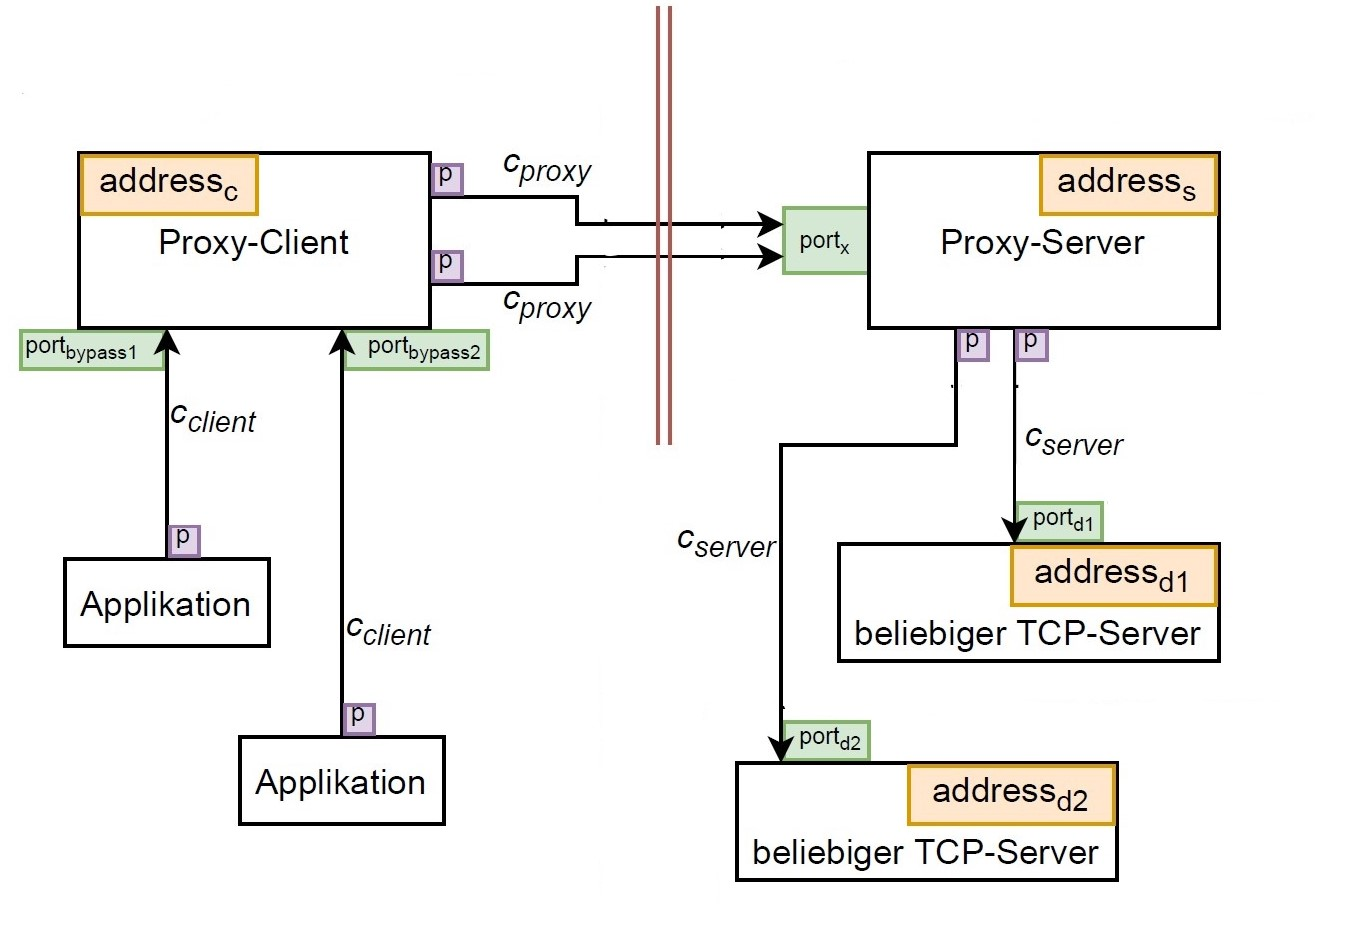
\includegraphics[width=0.75\linewidth]{entities.jpg}
    \caption{Netzwerk-Architektur to bypass a firewall}
    \label{fig::arch}
\end{figure}

\newpage
\section{Security}
At the end of task 1 the proxy system parses a configuration file, accepts multiple requests at a time and in general is fully functional. Nerveless it still lacks some basic requirements in terms of security and availability. The following section discusses these and all involved entities.

\subsection{Entities}
The following entities are involved by using the proxy:
\begin{figure}[H]
    \centering
    \begin{subfigure}{0.45\textwidth}
        \begin{itemize}
            \item User:
            \begin{itemize}
                \item Application
                \item ProxyClient
            \end{itemize}
            \item Proxy-Provider
            \begin{itemize}
                \item ProxyServer
            \end{itemize}
            \item Content-Providers
            \begin{itemize}
                \item E-Mail
                \item WebServices
                \item PrivateServices
                \item \ldots
            \end{itemize}
        \end{itemize}
    \end{subfigure}
    \begin{subfigure}{0.5\textwidth}
        \centering
        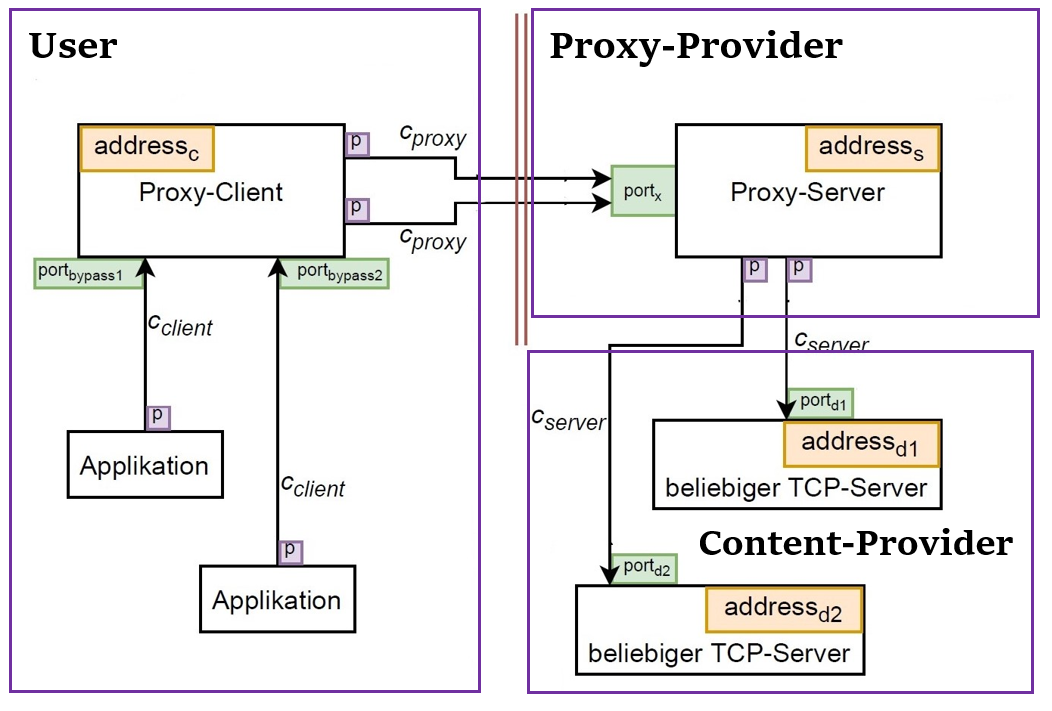
\includegraphics[width=\linewidth]{entities.png}
        \caption{Entities of the proxy client-server setup}
        \label{fig::enti}
    \end{subfigure}
\end{figure}

\noindent Each entity runs one or more technical entities. Technical entities are the processes that a entity operates on.\newline
The following section discusses the relation between these entities as well as the security risks that exists in-between them.
\subsection{Security risks and restrictions}
\paragraph{User \& ProxyProvider:}\label{ssec::user}
\noindent Any internet connected device can perform requests to the proxy. The server can not be sure that the client that connects is indeed a valid client instead of a malicious client that spoofs its identity. The same problem persists on the client side. Attackers may fake the proxy client and convince users to connect to their server and perform further malicious actions. There is no way the entities can be sure about each others identity and thereby it violates the principle of \textbf{Authentication}.\newline
Some parts of the communication infrastructure are owned by third party entities. Every one that has access to a part of the communication infrastructure can capture all confidential information on that infrastructure and use it against the recipient. This violates the principle of \textbf{Confidentiality}.\newline
Beside capturing information it is also possible to alter the information wich violates the principle of \textbf{Integrity}.
\paragraph{ProxyProvider \& Content-Providers:}
The proxy server provide allows strangers to access his services and also redirects any request to other services. So the server provide may be responsible for attacks on third-party services that are caused by abusive usage of his server.\newline
The proxy infrastructure itself can be a potential target. Too many request or bad requests (like a \ac{DoS} attack) could crash the proxy server and make it unavailable for all users.
\paragraph{User \& Content-Providers:}
As already described in \@\ref{ssec::user}, in the current configuration there is no confidentiality between any of the entities. The technical cause for that is that the currently used sockets don't support the \ac{TLS} protocol. Even if the application or the destination support \ac{TLS} it doesn't work because the authentication and key exchange between proxy and endpoint fails. With this restriction the user is limited to unencrypted services such as \acs{HTTP}.
\subsection{Possible solutions}
\paragraph{Confidentiality, Integrity and Authentication}
To ensure that the user connects to a valid proxy server one could introduce certificates for authentication. The server identifies itself with a certificate that is verifiable by the client. This solves the previously nonexistent \textbf{Authentication}. The same principle could be be applied to also allow the authentication of the client to the server. For this the server must own all CA-certificate that signed to clients certificates or all clients must be distributed with progenerated certificates.\newline
The certificate exchange and technical authentication would happen within the \ac{TLS} handshake. With the certificate and their keys it is also possible to encrypt messenges with \ac{TLS}. This would ensure the \textbf{Confidentiality} of any message. The encryption algorithm depends on the version and configuration of \ac{TLS}.\newline
To ensure \textbf{Integrity} it is possible to hash the message, encrypt the hash and append it to message as signature. The recipient can compare the hash he calculated with the decrypted hash of the sender. If both hashes match it guarantees the integrity of the message.\newline
The technical implementation of \ac{TLS} is done in the \ac{SSL} python module.
\paragraph{Availability and abuse protection}
In addition to the security of communication, the availability of the services must also be ensured. This is feasible with a access control to specific user or resource limits for requests and compute time. Loadbalancers and backup systems could improve availability even further.\newline
These actions and an additional blacklist for specific services could also help to protect the server against abusive or illegal usage.

\section{Evaluation}
In the context of this evaluation, only the throughput of the proxy is considered, other metrics such as delay and packet loss are neglected.
\subsection{Testsetup}
\begin{figure}
    \centering
    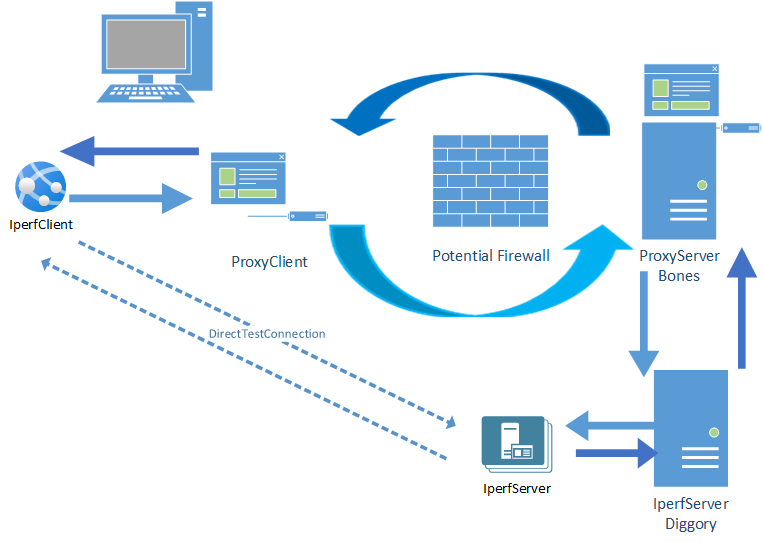
\includegraphics[width=0.45\linewidth]{TestSetup.png}
    \caption{Throughput test setup}\label{fig::test}
\end{figure}
The throughput measurements where made with the \code{iperf} tool. All nodes (client(Vogon), TestServer1(diggory), TestServer2(bones)) are running Linux (Kali 2020.3 on Vogon, Ubuntu 14.04 on diggory/bones) and version 2.0.14a of \code{iperf} on the client and version 2.0.5 on the server. The \code{iperf} server and client is running mostly in standard configuration except for more verbose logging (0.5s interval) and a fixed amount of data to transmit instead of a fixed test duration of 10 seconds. An exemplary call for client and server can be found in listing \ref{code::iperf}. Results with the fixed data setting makes it easier to approximate download times for in use cases and is also easier interpretable for non technical readers.\newline
The test only covers the download throughput. Because the client is behind a NAT and has now way to expose its IP it was not possible to perform a bidirektional test.\newline
The baseline throughput test is a direct connection between the \code{iperf} client (Vogon) to diggory without any proxy. Now diggory runs the proxy server and Vogon starts the porxy client. Iperf now connects to the proxy client which redirects the connection to bones and for there to the destination \code{iperf} server on diggory. This setup with these three nodes represent a realistic usage of the proxy in production. A systematic structure of this setup is shown in fig.\@\ref{fig::test}.\newline
The proxy was tested with a SSHProxy, noSSL, server-authentication, client-server-authentication and client-server-authentication configuration with \ac{ACL}. Each test runs 15 iterations of every configuration. In total the test was performed eight times each with 6 hours interval. The script for the exact test can be found with the resources of this paper.
\subsection{Analysis of the results}
Each generated log was parsed with a custom script wich also generated the following grafics.

\begin{figure}
    \centering
    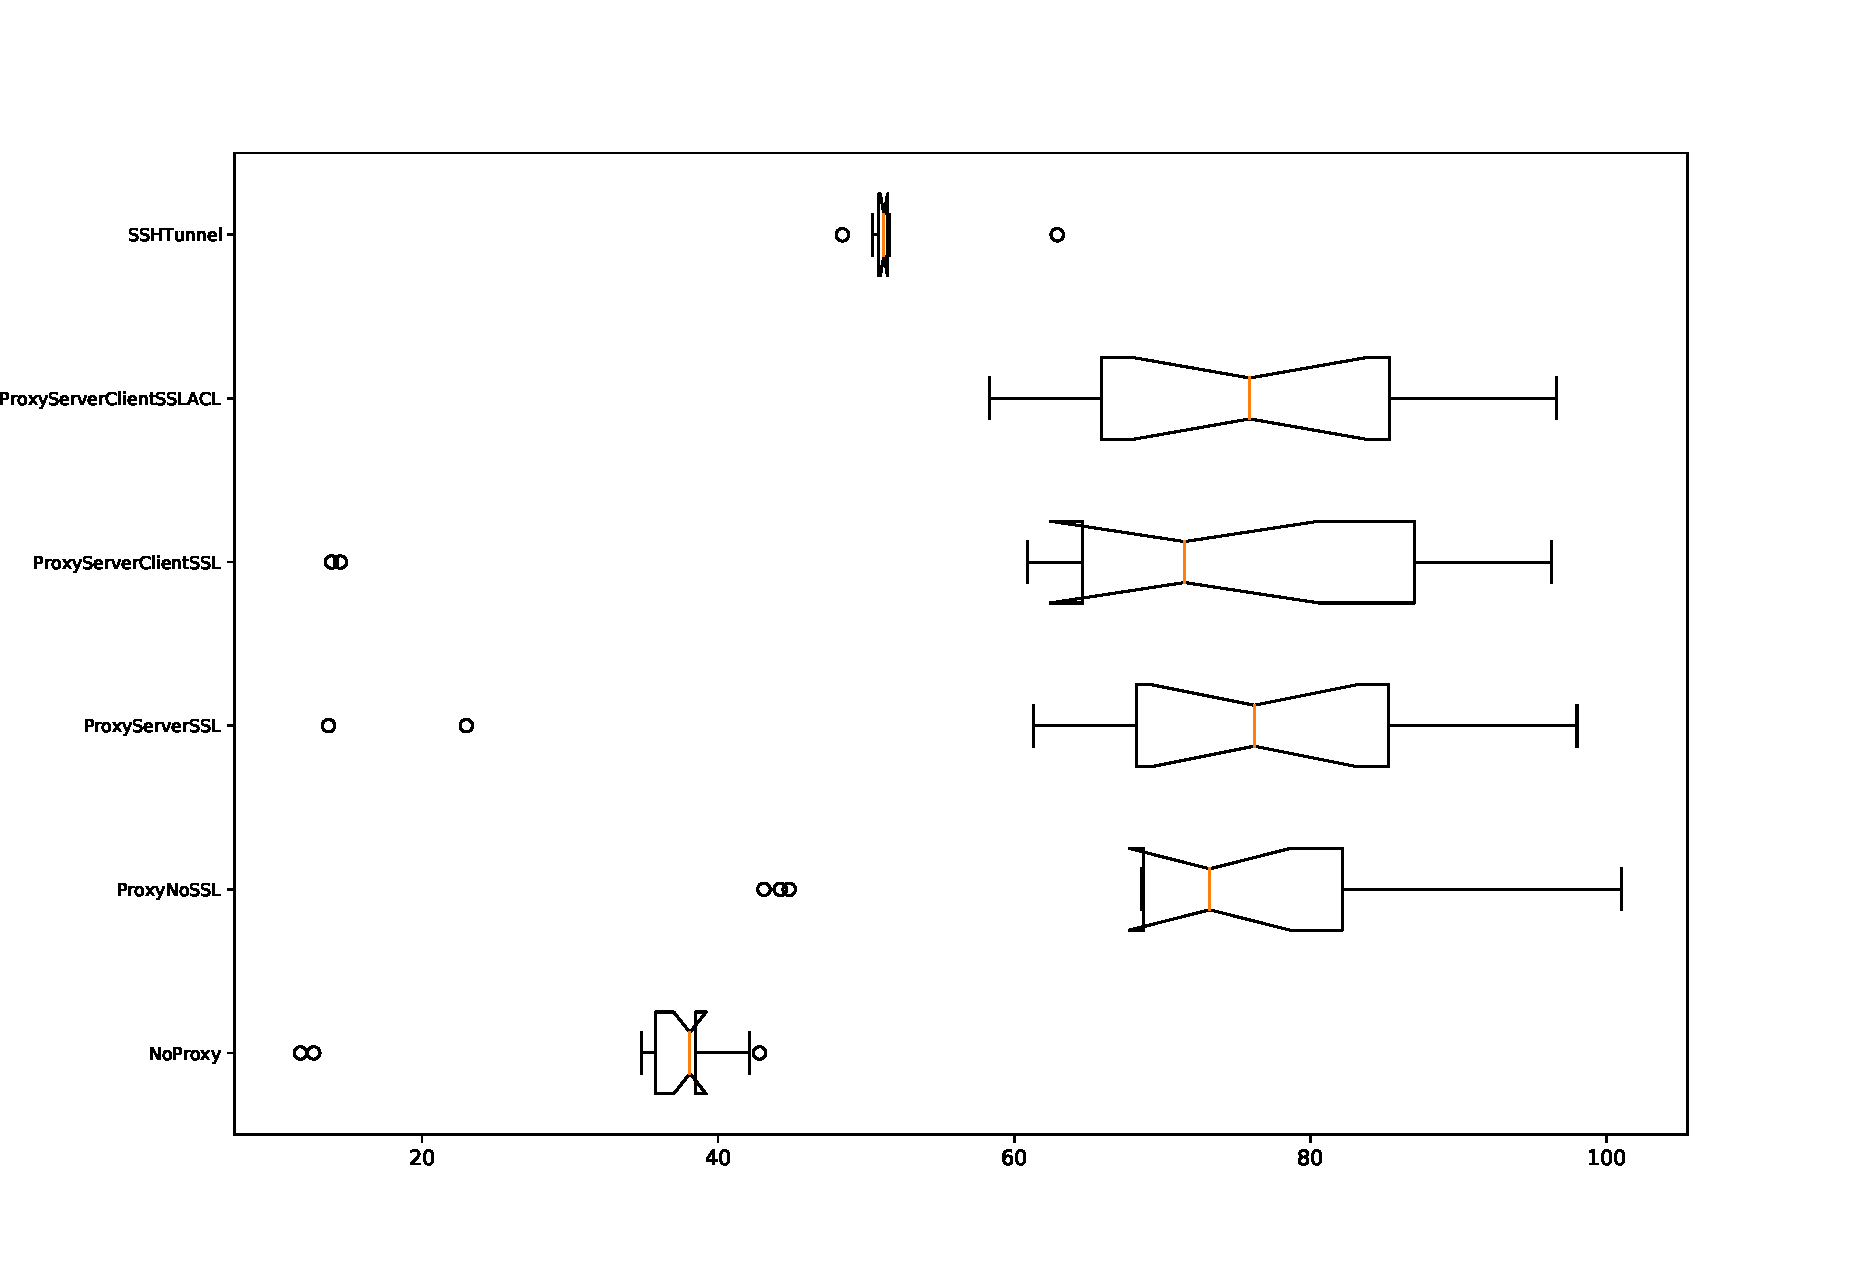
\includegraphics[width=0.95\linewidth]{boxplot.pdf}
    \caption{Throughput test results}\label{fig::boxres}
\end{figure}
\noindent Figure \@\ref{fig::boxres} shows the results of the throughput test performed with \code{iperf}. Contrary to expectations, the direct connection (vogon to diggory) without a proxy delivers the worst throughput with an average of 35.81 Mbit/s. To eliminate as many variations as possible the test was also performed with the \code{-N} flag for \code{iperf} to disable kernel package buffering. This did not change the results.\newline
During the tests, if the test were canceled, it was found that the data throughput was very high (Gbit/s). This happend when \code{iperf} assumes that the packages where already acknowledged when in fact the server did not receive anything. This did not happen during valid tests, as one could see from the monitored server logs. Lowering the receive buffer size in the proxy resulted in fact in a decreased throughput, after this change and additional checks with Wireshark, the possibility of an implementation error was rejected. The results form the SSHTunnel, that did not run self implemented code, support this assumption. It is presumed that \code{iperf} could already use the acknowledged of the proxy client to calculate the throughput and thus does not represent the real speed. After all this behavior needs further investigation to allow for final statements.\newline
All other proxy configurations provide an average throughput between 71.5 and 77.7 Mbit/s. With a slight deterioration in \ac{SSL} configurations due to additional \ac{SSL} overhead. This is still 2x the throughput without any proxy at all. The variation in speeds, per configuration also provides some findings. The direct test without any proxy and the test with the SSHTunnel provide the most consistent throughput.\newline
This throughput evaluation shows that the proxy throughput is more than enough for simple web-browsing. Unsupervised practical tests also show usability for video streaming. The additional latency caused by the proxy, which could influence the usability of real-time applications, was not measured in this test. The additional latency caused by the proxy, which could influence the usability of real-time applications, was not measured in this test. This should be investigated at a later date.

\subsection{Conclusion}
The implemented proxy setup allows it to bypass a firewall and thereby fulfills its purpose. With the use of \ac{SSL}, it can also be used practically without running the risk of disseminating all of its information unprotected in the network. ClintSide authentication introduces a lot of additional configuration work and should be only be used in embedded applications. ServerSide authentication is recommended and is much easier to setup.\newline
Submitting a config file for one specific goal also makes usability more difficult. This shows the advantages that the SOCKS protocol provides. Web-browsing and applications that require a moderate bandwidth are, however, possible without problems with the proxy. Realtime application like \ac{VoIP} or gaming may suffer from the additional latency and the less consistent connection.\newline
Depending on use case this proxy can provide an acceptable solution accessing resources that would have been inaccessible otherwise.

% Anhang
\newpage
\renewcommand{\thesubsection}{\Alph{subsection}}
\pagenumbering{Roman}
\setcounter{page}{\value{lastroman}}
\section*{Appendix}
\addcontentsline{toc}{section}{Appendix}
%Abkürzungsverzeichnis
% !TeX root = ../ITS_WiSe_202021_Hausarbeit_969272.tex
\newcommand{\abbr}{Abbreviations}
\subsection{Abbreviations}
%\addcontentsline{toc}{subsection}{Abbreviations}

\begin{acronym}[1234567890]		%[längste Abkürzung]
\setlength{\itemsep}{-\parsep}	% sorgt dafür, dass das Verzeichnis kompakt dargestellt wird.

\acro{DoS}[DoS]{Denial of Service}
\acro{TLS}[TLS]{Transport Layer Security}
\acro{HTTP}[HTTP]{Hypertext Transfer Protocol}
\acro{ACL}[ACL]{Access Control List}
\acro{SSL}[SSL]{Secure Sockets Layer}
\acro{VoIP}[VoIP]{Voice over IP}

\end{acronym}
%Code
% !TeX root = ../main.tex
\subsection{Iperf test script}
\begin{lstlisting}[frame=single, language=bash, caption={Iperf test script},label=code::iperf]
#!/bin/bash

ITERATIONS=15
PACKAGE_SIZE=16MB
SERVER="diggory"
LOG_FILE="iperf_${SERVER}_new_1.log"

# Example server call
# iperf -s -i 0.5 -N -p 2622

for iteration in $(seq 1 $ITERATIONS); do
    echo "NoProxy" >> $LOG_FILE
    iperf -c ${SERVER}.informatik.uni-osnabrueck.de -i 0.5 -p 2622 -n $PACKAGE_SIZE -N >> $LOG_FILE

    echo "ProxyNoSSL" >> $LOG_FILE
    iperf -c 127.0.0.1 -i 0.5 -p 8000 -n $PACKAGE_SIZE -N >> $LOG_FILE

    echo "ProxyServerSSL" >> $LOG_FILE
    iperf -c 127.0.0.1 -i 0.5 -p 8001 -n $PACKAGE_SIZE -N >> $LOG_FILE

    echo "ProxyServerClientSSL" >> $LOG_FILE
    iperf -c 127.0.0.1 -i 0.5 -p 8002 -n $PACKAGE_SIZE -N >> $LOG_FILE

    echo "ProxyServerClientSSLACL" >> $LOG_FILE
    iperf -c 127.0.0.1 -i 0.5 -p 8003 -n $PACKAGE_SIZE -N >> $LOG_FILE

    echo "SSHTunnel" >> $LOG_FILE
    iperf -c 127.0.0.1 -i 0.5 -p 2222 -n $PACKAGE_SIZE -N >> $LOG_FILE
done
\end{lstlisting}
\newpage
\listoffigures
% !TeX root = ../main.tex
\section*{Declaration of Authorship}

\vspace{5cm}

~\\
I hereby declare that the paper submitted is my own unaided work. I assure that I wrote this paper without using any other means and sources than those specified. As well as the sources used literally or analogously taken from the sources identified as such.

\vspace{3cm}
\begin{flushright}

\rule{8cm}{0.2mm} \\
Signature (\myName)
\end{flushright}

\vspace{2cm}
\place, the \submission{}

\end{document}
